%%% 第三章
\chapter{吸收塔内部附件的选择}
填料塔内件是填料塔的重要组成部分,它们的设计和选择对填料塔的性能有着直接的影响。填料塔内件的设计需要考虑多种因素,包括塔的直径、操作压力、处理的物料性质、填料的类型和特性等。设计时还需要确保内件能够提供足够的强度和刚度,以承受操作中的压力波动、机械震动和温度变化。此外,内件的设计应促进气液的均匀分布,以提高传质效率和塔的整体性能。



%%% ===============================================
\section{液体分布器的选择}
液体分布器是填料塔中的关键内件,它的主要作用是将液体均匀地分布在填料层的顶部,或者在塔内的某一高度上进行再分布。液体分布器的性能直接影响填料的传质效率和操作弹性。合理的液体分布可以减少填料塔内的放大效应和端效应,提高塔的整体效率,减少塔的尺寸和造价。

液体分布器的工作原理是通过其设计的结构,将进入塔内的液体以均匀的方式分配到填料层上,确保液体能够在填料表面形成均匀的膜状流动,从而实现有效的气液接触和传质。设计要求包括液体分布均匀、操作弹性大、结构紧凑、气体流通面积大、具备液体收集、分布及气体分布功能等。

液体分布器的类型多样,可以根据其流体动力特性、形状、液体离开的形式、分布的次数以及组合方式进行分类。例如,按分布器流体动力分有重力型和压力型,按形状分有管式、槽式、盘式等,按液体离开形式分有孔流型和溢流型。液体分布器的选择依据主要包括分布质量、操作弹性、处理量、气体阻力、对水平度等多个方面。

为了确保液体分布器的正常运行和填料塔的高效操作,需要定期检查分布器的工作状态,包括液体分布的均匀性和压降。在维护时,应注意检查是否存在堵塞或磨损,并及时进行清理或更换。优化建议可能包括调整液体分布器的设计以适应特定的操作条件,或者采用新型抗堵塞的设计来提高塔内的操作弹性和减少维护工作量。

槽式液体分布器具有较大的操作弹性和极好的抗污堵性,特别适合于大气液负荷,应用范围非常广泛。所以本次\ce{SO2}设计中选用槽式液体分布器。

\clearpage

\begin{figure}
	\caption{槽式液体分布器示意图}
	\centering
	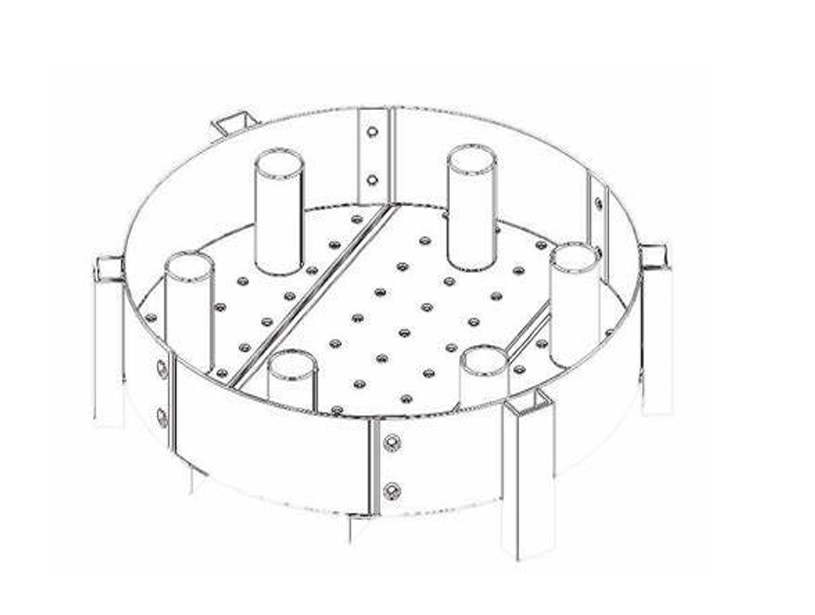
\includegraphics[width=\textwidth]{槽式液体分布器.png}
\end{figure}



%%% ===============================================
\section{液体再分布器的选择}
再分布器采用升气管式设计,适合大直径塔体。
除塔顶液体的分布之外,填料层中的液体的再分布是填料塔中的一个重要问题。往往会发现,在离填料顶面一定距离处,喷淋的液体便开始向塔壁偏流,然后雁塔壁下流,塔中心处填料得不到好的湿润,形成所谓“干椎体”的不正常现象,减少了气液两相的有效接触面积。因此每隔一定距离必须设置液体再分布器,以克服此种现象。升气管式再分布器适用于直径0.9 m以上的塔,而且可以分段卸下填料,更换填料方便,所以本设计选用升气管式再分布器



%%% ===============================================
\section{填料支承装置的选择}
填料支承装置的作用是支承填料以及填料层内液体的质量,同时保证气液两相顺利通过。支承若设计不当,填料塔的液泛可能首先发生在支承板上。为使气体能顺利通过,对于普通填料塔,支承件上的流体通过的自由截面积为填料面的50\%以上,且应大于填料的空隙率。此外,应考虑到装上填料后要将支承板上的截面堵去一些,所以设计时应取尽可能大的自由截面。自由截面太小,在操作中会产生拦液现象。增加压强降,降低效率,甚至形成液泛。由于填料支承装置本身对塔内气液的流动状态也会产生影响,因此作为填料支承装置,除考虑其对流体流动的影响外,一般情况下填料支承装置应满足如下要求:

足够的强度和刚度,以支持填料及所持液体的质量(持液量),并考虑填料空隙中的持液量,以及可能加于系统的压力波动,机械震动,温度波动等因素。

足够的开孔率(一般要大于填料的空隙率),以防止首先在支撑处发生液泛;为使气体能顺利通过,对于普通填料塔,支承件上的流体通过的自由截面积为填料面的50\%以上,且应大于填料的空隙率。此外,应考虑到装上填料后要将支承板上的截面堵去一些,所以设计时应取尽可能大的自由截面。自由截面太小,在操作中会产生拦液现象。增加压强降,降低效率,甚至形成液泛。

结构上应有利于气液相的均匀分布,同时不至于产生较大的阻力(一般阻力不大于20Pa)。本设计运用 的瓷质鲍尔环,孔隙率相对较大,升气管式支撑板能更好的克服支撑板的强度和自由截面之间的矛盾,耗能更好的适应高空隙率填料的要求,本设计选用升气管式支撑板。



%%% ===============================================
\section{填料压紧装置的选择}
填料支撑是填料塔内部的一个重要组成部分,它的主要作用是支撑填料层,确保填料在塔内均匀分布,防止填料在操作过程中发生下沉或移动,从而维持填料层的结构稳定性和传质效率。填料支撑还能够承受塔内的压力和机械负荷,保护塔体结构不受损害。

填料支撑的类型包括栅板式支撑、压板式支撑和驼峰支撑等。栅板式支撑通常由金属材料制成,具有一定的空隙率,可以放置在塔的支承圈上。压板式支撑则是制成栅板形状的填料压紧器,依靠自身重力将填料压紧。驼峰支撑则是通过冲压、切割等方式制成的立体结构,具有良好的力学性能和流体力学性能。

驼峰型支撑装置具有高刚性与载荷能力、优良流体分布性、节省材料,降低塔体重量,提升操作弹性和处理能力等优点。所以本次SO2吸收设计中选用驼峰型支撑装置。

压紧装置的作用是在填料塔操作过程中,通过施加压力来确保填料层的紧密性和稳定性。压紧装置通常安装在填料层的上方,可以是简单的重力式压紧,也可以是带有弹簧或其他机械装置的压紧系统。压紧装置的设计要能够适应不同操作条件下的压力变化,确保填料层在高压降或负荷波动时不会松动或破损。

为了确保填料支撑和压紧装置的正常运行,需要定期检查其结构的完整性和压紧效果。在维护时,应检查支撑结构是否有变形、腐蚀或损坏,并及时进行修复或更换。优化建议可能包括使用高质量的材料来提高支撑和压紧装置的耐久性,以及根据操作条件调整压紧力度,以达到最佳的传质效果和塔的运行效率。

填料压紧网板的设计要求有足够的空隙率,通常大于70\%,可以减少流体阻力并促进气液的均匀分布和防止填料从间隙中漏出。所以本次SO2吸收设计采用填料压紧网板。



%%% ===============================================
\subsection{除沫装置}
除沫装置在化工、石油等行业的塔器设备中起着至关重要的作用。它的主要功能是从气体流中去除夹带的液滴,以提高塔内的传质效率,减少物料损失,保护下游设备如压缩机不受液沫侵蚀,延长设备寿命,并减少环境污染。在气体吸收过程中,除沫装置还能保证气体的纯度,使后续过程能正常运行。

除沫装置的类型包括丝网除沫器、折流板除沫器和旋流板除沫器等。丝网除沫器利用丝网的比表面积大、空隙率高的特点,通过气体与丝网的碰撞和惯性作用来分离液滴。折流板除沫器和旋流板除沫器则利用气流在板上的旋转运动产生的离心力来分离液滴。这些装置通常安装在塔的顶部或其他需要气液分离的位置。

除沫装置的设计要点包括高效率的除沫、小的压力降、抗堵塞能力以及结构的简单性。优化方法可能包括改进丝网的材料和结构,以提高除沫效率和抗堵塞能力,或者优化旋流板的设计以提高分离效率和降低阻力。

抽屉式丝网除沫器是一种经济型除沫装置,它采用标准的丝网除沫元件,可以在塔体外更换,便于操作和维护。这种除沫器的特点是阻力低,可反复清洗,经济性高,且结构简单,投资少。此外,这种除沫器还具有较高的除沫效率和较小的压力降,有利于提高设备的生产效率。所以本次\ce{SO2}吸收设计选用抽屉式丝网除沫器。